\documentclass[a4paper,12pt]{article}
\usepackage{amsmath}
\usepackage{amsfonts}
\usepackage[english]{babel}
\usepackage{fancyhdr}
%\usepackage[prefix]{nomencl}
%\usepackage{makeidx}
\usepackage{cite}
\usepackage{float}
\usepackage{placeins}
\usepackage{graphicx}
\usepackage{epstopdf}
%\usepackage{multicol}
%\usepackage{url}
\usepackage{listings}
\usepackage{pdfpages}
\usepackage[utf8]{inputenc}
\usepackage[hidelinks]{hyperref}
%\usepackage{cleveref}

\usepackage{caption}
%\usepackage{subcaption}
\usepackage{subfig}
\renewcommand{\contentsname}{Innehållsförteckning}
%\hypersetup{linkcolor=blue, colorlinks=true}


%\makenomenclature

\let\oldAuthor\author
\renewcommand{\author}[1]{\newcommand{\myAuthor}{#1}\oldAuthor{#1}}
\renewcommand{\deg}{\ensuremath{^{\circ}}\xspace}

\begin{document}

%---------------------------------------------------------
%Fill in:
% Redaktör
%---------------------------------------------------------

%---------------------------------------------------------
%Fill in:
%1. Redaktör(er)
%3. Organisation/Företag/Institution...
%4. Projektnamn
%5. Projektgrupp, med email eller liknande kontakt uppgift
%6. Granskare av dokument
%7. Datum som graskningen skedde
%8. Godkännare av dokumentet
%9. Datum för godkännande
%---------------------------------------------------------
\title{Project report}
\author{Tobias Nilsson \\ Jesper Vesterberg}
\date{} %<-- LEAVE EMPTY! 
\newcommand{\organisation}[0] {\small Institutionen för Fysik \\ Umeå Universitet}
\newcommand{\projektnamn}{\small Upgrade: Electrical Conductivity}
\newcommand{\projektgrupp}{ Tobias Nilsson, \\ toni0042@student.umu.se \\
							 Jesper Vesterberg,\\ jeve0100@student.umu.se}
\newcommand{\granskare}{Jesper Vesterberg}
\newcommand{\granskatdatum}{GRANSKATTDATUM}
\newcommand{\godkannare}{Krister Wiklund}
\newcommand{\godkantdatum}{GODKÄNTDATUM}


\begin{titlepage}
\maketitle 
\thispagestyle{fancy}
\headheight 35pt 
\lhead{\organisation}
\chead{\projektnamn}
\rhead{\small\today}
\cfoot{\projektgrupp}

\begin{center}
Version 1.0
\end{center}

\vspace{80mm}
\begin{center}
  {\large Status:}\\[1.5ex]
  \begin{tabular}{|*{3}{p{40mm}|}}
    \hline
    Reviewed & \granskare & \granskatdatum \\
    \hline
    Approved & \godkannare & \godkantdatum \\
    \hline
  \end{tabular}
\end{center}

\end{titlepage}



\pagestyle{fancy}
\headheight 35pt 
\pagenumbering{roman}
\rhead{\small\today \\ }
\chead{\projektnamn}
\lhead{\organisation \\ }
\lfoot{Projektarbete inom \\teknisk fysik B, 3.0 HP \\ 5FY070}
\cfoot{\thepage}
\rfoot{\projektgrupp}
\begin{center}

\section*{\center Project identity}

\bigskip
\begin{tabular}{|p{35mm}|p{30mm}|p{20mm}|p{45mm}|}
\hline
\textbf{Name} & \textbf{Ansvar} & \textbf{Telephone} & \textbf{e-mail}\\
\hline
Tobias Nilsson & Documents &  & toni0042@student.umu.se\\
\hline
Jesper Vesterberg & Programmer &  & jeve0010@student.umu.se\\
\hline
\end{tabular}

\bigskip
\textbf{Client}: Institutionen för Fysik, Umeå universitet, \\
Linnaeus väg 24,\\
901 87\\
Umeå.

\textbf{Contact}: Krister Wiklund, krister.wiklund@umu.se.
\end{center}
\newpage

\tableofcontents
\newpage
\pagenumbering{arabic}

\section{Introduction}
The purpose of the lab \emph{Electrical conductivity} in the courses \emph{Solid State Physics} is to investigate how the electrical conductivity of different materials behaves in the temperature region $10-300$ $K$. The materials in question are a semi-conductor, InSb, a metal, Pt, and a super conductor, $YBa_2Cu_3O_7$.

The aim of the project was to upgrade the the laboratory equipment, which consisted of; a cryo system, with heat controller; a series of power supplies; a black box with measurement circuits, that converted resistance to voltage; a bench multimeter and an ancient  computer system running on MS-DOS. The upgrades consisted of removing the external power supplies, the black box, exchanging the computer for a newer laptop and the user interface, \emph{Elledn}, was rewritten in Labview.



\section{The set-up}
Equipment consist of:
\begin{itemize}
\item Cryogenic system:
\begin{itemize}
\item Cooling chamber
\item Coarse vacuum pump
\item Turbo molecular pump
\item Cryogenic system(compressor w. cooling system): HC-2, APD Cryogenics Inc.
\end{itemize}
\item Controllers to cryogenic system: 
\begin{itemize}
\item Turbotronic NT10
\item Thermovac TM20
\item Scientific Instruments Inc. 9620-1 Silicon Diode
\end{itemize} 
\item Bench Multimeter: Keithley 2001 Multimeter
\item Computer with Labview.
\end{itemize}

The materials are placed in the cooling chamber and the two vacuum pumps reduces the pressure to below $10^{-5}$ Pascal. This reduces the amount of heat that needs to be removed to change the chambers temperature. Remember the ideal gas law $PV=NkT$. The actual cooling process is a closed helium-gas cycle that follows the Gifford-McMahon principle.

The samples are continuously cooled by the equipment to $\approx 10$ $K$ if no additional heat is added. Thus to change the temperature additional heat is added to the system by an external heater. This heater is controlled by the \emph{Scientific Instruments Inc. 9620-1 Silicon Diode}. Which in turn can be controlled by a computer through an GPIB-interface and its front panel. 

The controller determines the heating with the aid of the PID equation, consisting of a \textbf{P}roportional, an \textbf{I}ntegral and a \textbf{D}ifferential term. To improve the performance and responsiveness of the cryogenic equipment in various temperature ranges, the coefficients for these terms can be changed by the user. For more information see equation \eqref{eq:PID} and the \emph{Scientific Instruments Inc. 9620-1 Silicon Diode manual}.

To determine the resistivity of the samples, each sample is connected to a 4 sense wire system. These sense wires are connected to a Keithley 2001 Multimeter through a switching card at the back of the multimeter. The multimeter is also equipped with a GPIB-interface, enabling computer controlled measurements. 

The connections from the samples and an additional temperature diode, goes first a through a round 19 pin contact to an 25 pin d-sub connector. See table \ref{tab:PinNumbers} for pin layout on the cables.

\begin{table}[H]
	
  \caption{\emph{Pin layout for connection cables between cooling chamber and multimeter. Ports 19-24 on the 25-pin Dsub connector are  unused.}} 
  
  \begin{tabular}{c|c|c c c}
  \label{tab:PinNumbers}
  25-pin D-sub & round 19-pin connector & Function & & \\
  \hline
  1  & A & Superconductor    & Current & + \\
  2  & B & ''                & ''      & - \\
  3  & C & ''                & Voltage & + \\
  4  & D & ''                & ''      & - \\
  5  & E & Conductor, Pt-100            & Current & + \\
  6  & F & ''                & ''      & - \\
  7  & G & ''                & Voltage & + \\
  8  & H & ''                & ''      & - \\
  9  & J & Semi-conductor, InSb-plate        & Current & + \\
  10 & K & ''                & ''      & - \\
  11 & L & ''                & Voltage & + \\
  12 & M & ''                & ''      & - \\
  13 & N & Temperature diode & Current & + \\
  14 & P & ''                & ''      & - \\
  15 & R & ''                & Voltage & + \\
  16 & S & ''                & ''      & - \\   
  17 & T & free              &         &  \\
  18 & U & free              &         &  \\
  25 & V & Shield            &         &  \\ 
  \end{tabular}
  
\end{table} 




The samples are connected to the Keithley Multimeter through a custom scanning card. This card enables the use of the built-in switching capabilities and it has two rows of pins, a red (positive) and a black (negative). When using this home made card for 4-wire measurements it can be important to know that the first five pins (pins 1-5) are used for the potential wires and that the  last five (pins 6-10) are used for the current wires.

The first potential pins are grouped with the first current pins, e.g. pins 1 and 6 are connected two sample 1 and pins 2 and 7 are connected to sample 2 and so on. See Table \ref{tab:ScanCard} for details about how the samples currently are connected to the scanning card.
 
 
 \begin{table}[H]
	\center
	
	\caption{\emph{Pin layout for the Scan card, inside the Keithley Multimeter.}} 
	\begin{tabular}{l|l|l}
	\label{tab:ScanCard}
		\#  & +(Red) & -(Black) \\
		\hline
		1  & Superconductor, Potential +	& Superconductor, Potential - \\
		2  & Semi-conductor, Potential +		& Semi-conductor, Potential - \\
		3  & Conductor, Potential +			& Conductor, Potential - \\
		4  & 	N/A	& N/A \\
		5  & 	N/A	& N/A \\
		6  & Superconductor, Current +		& Superconductor, Current - \\
		7  & Semi-conductor, Current +		& Semi-conductor, Current - \\
		8  & Conductor, Current +			& Conductor, Current - \\
		9  & 	N/A	& N/A \\
		10 & 	N/A	& N/A \\
	\end{tabular}
	
\end{table}

\section{Software}

This section describes shortly how the software works. For a guide on how to operate the software see the laboratory instructions for electrical conductivity. 

The software, ResSolidLabV1 (see figure \ref{fig:UI} for a snap shot), is written in Labview and its user interface has a reduced control of the measurement system. For simplicity it can only change the temperature and initiate measurements. All other changes in the measurement system, has to be done outside the user interface. Such as changing the different coefficients in the PID equation that controls the heating element. 


\begin{figure}[H]
	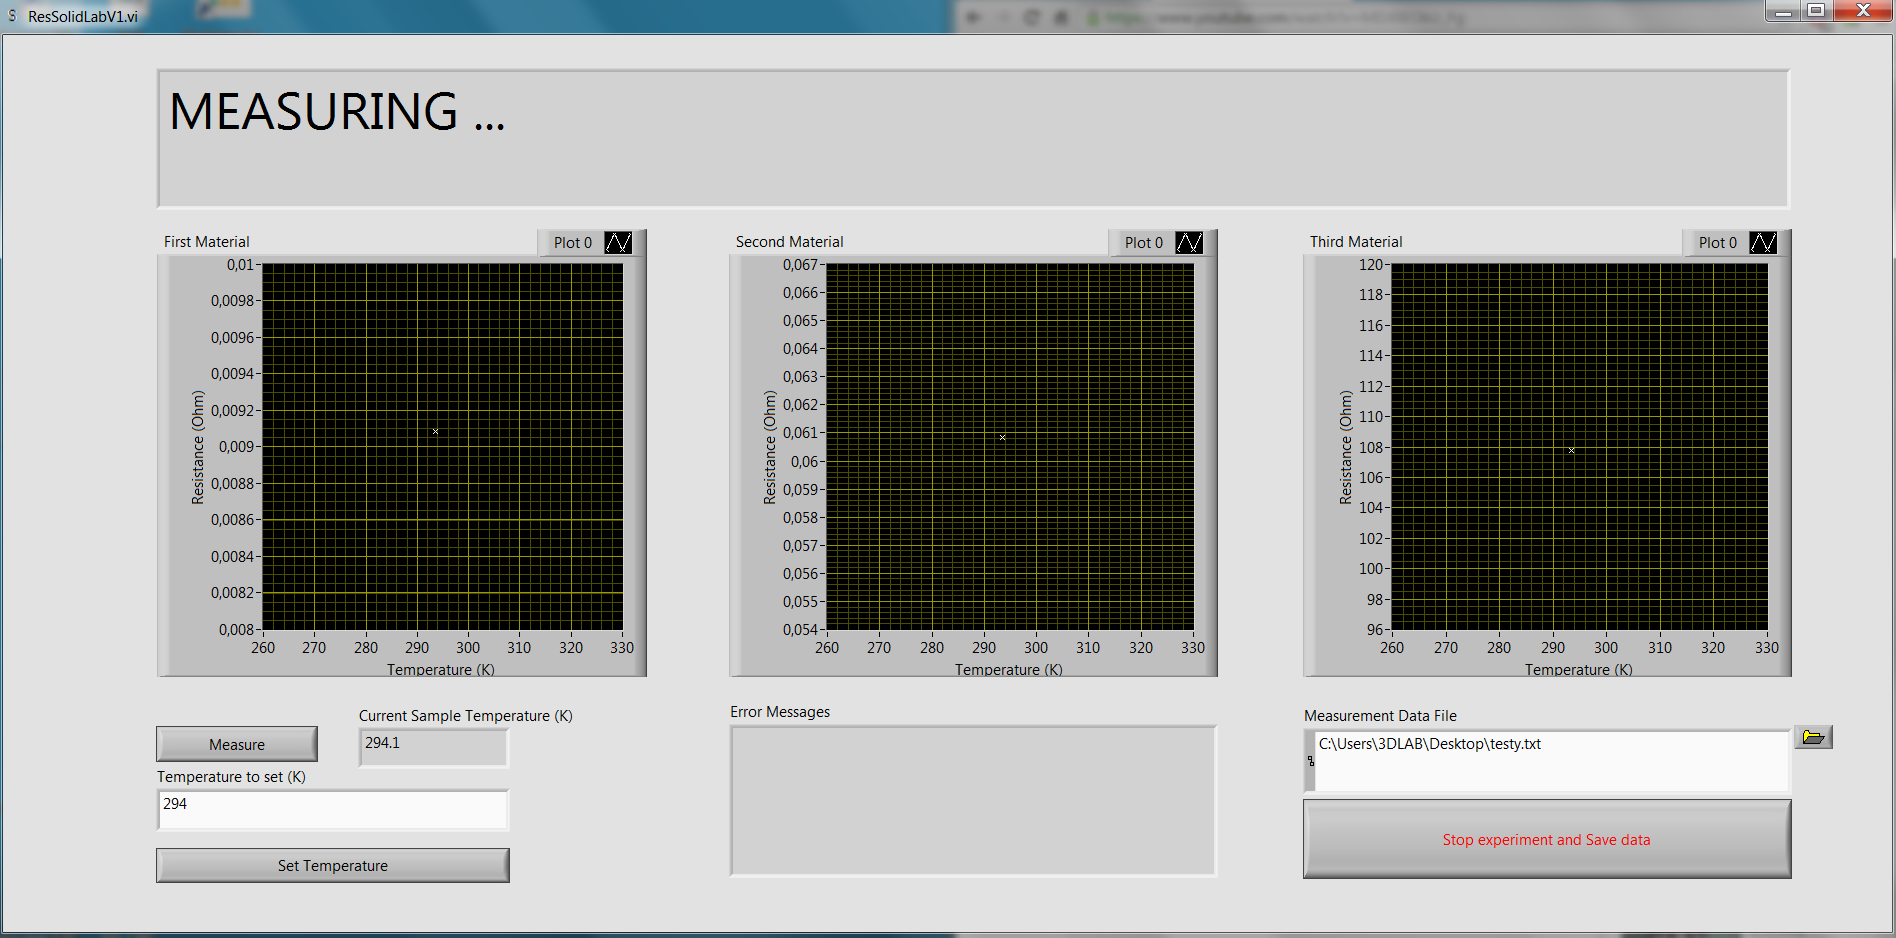
\includegraphics[width=1\textwidth]{ResSolidLabV1UI}
	\caption{\emph{Snapshot of the ResSolidLabV1's user interface.}}
	\label{fig:UI}
\end{figure}

However the bench-multimeter's settings are made automatically by ResSolidLabV1, these settings are about how the measurements are performed and the change these settings, the parts of the program needs to be rewritten.

The  bench-multimeter can not truly measure zero resistance even with the 4-wire setup and the measured values are often negative. The solution implemented in the software is to chose the maximum value between the measured resistance and zero. This introduces a potential problem. Switching place of either the current or resistance cables will change the sign of the measure resistance.

\subsection{Installation}
Description of how the installation is done. Note that the drivers for the GPIB usb interface is included in the installation and that a labview runtime is also included. Thus nothing else but the program itself needs to be installed.

\section{Doing Proper Measurements}
In order to get good measurements the old setup had a black box which was used to create a reverse-current measurement of the voltage drop over the samples in the cooling chamber. The voltage drop was measured by the keithley multimeter and was then translated to resistance inside the computer. This could be calculated since known calibration resistance measurments was also done inside the black box. Ontop of this the four wire measurement was made between the black box and the samples but not between the multimeter and the black box.

First of on the subject of reversal of current. This is made so that all currents created due to thermocoupling (i.e. in the interface of two different metals) is removed. But there can still be offsets due to non-ohmic contacts. This on the other hand does not affect the characteristics of the measurements, which is the thing this laboration focus on. A different method, and perhaps better method since it takes away offset due to non-ohmic contacts, is to use offset compensation. Basically you measure the residual voltages after a measurement and remove that offset instead.

By removing the black box and make four wire resistance measurments directly from the multimeter onto the samples we remove problems that can occour in between the multimeter and black box. The multimeter also have internal functions to do offset compensation which makes the measurments as good if not better, since stuff like not perfect dc voltage in the black box due the nature of AC power will have less effect on the measurement. It also makes the setup itself allot simpler.  

\section{Hardware Setup}
\subsection{How Measurements Are Done}
All measurments are done over the GPIB interface. All GPIB commands required for the measurements are done in the background by the ConductiveSolidLab program. First of it sets the temperature if you click the "set temperature" button and continously poll the temperature controller to see what the current temperature is in the "Current Sample Temperature (K)" window. 

The resistivity measurments are more complicated. But basically when you hit the "Measure" button the program stops and speaks with the multimeter. Here the multimeter takes 10 measurements of each samples and the labview program averages this and writes the result to file and displays it in the plot windows for each sample. 

\subsection{Temperature Controller}
We have the temperature controller hooked up to the heating element in the cooling chamber and a diode for measuring the temperature. Sadly only one of the diodes seem to be functional so only one source is used to find the temperature. The temperature controller is then hooked up to a computer through its GBIB interface.

\subsubsection{GPIB commands used}
Note that all commands in this description list contains a {\textbackslash}r in the end. This is because labview automatically appends a newline (i.e. {\textbackslash}n) when it sends a GPIB command. The temperature controller on the other hand expects a carriage return \emph{and} a newline (i.e. {\textbackslash}r{\textbackslash}n).
\begin{description}
\item [T{\textbackslash}r] This command tells the temperature controller to send back the current temperature as a response 
\item [S00000{\textbackslash}r] This command sets the temperature the temperature controller should try and achive. The temperature is given in five integers and it is goes between the temperature of 0000.0 and 9999.9 Kelvin. All four digits must always be supplied. 
\end{description}

\subsection{Bench Multimeter}
We have a Keithley 2001 multimeter that does all of the resistance measurements. It is hooked up directly into the three samples and and can be controlled through its GPIB interface. For a complete reference to its GPIB interface you are refered to its operational manual. We will go through the commands made to make a measurement in this laboration setup.

\subsubsection{GPIB measurement}
The code for making the multimeter do proper measurement is quite substantial. Not because advance calculations has to be made, but the options on the Keithley 2001 multimeter is nothing but daunting when you first look at it. It has to have three layers configured, the initialization layer, ARM layer and Trigger layer before a measurment. Beyond this certain buffer sizes and registers need to be configured correctly in order for a proper measurment to be done that can be read programatically. It is also far from obvious what values to set what register to. One also has to configure the multimeter for four wire resistance measurments and offset compensation so one does not have to manually configure the multimeter every time the laboration is to be done, minimizing setup time and uneccessary problems due to a badly configured multimeter. 

To fully understand the code one must be familiar with the GPIB interface in general and the Keithley 2001 multimeter operation manual. This can be much, so the code has been written as clearly as possible so that just passing understanding of these things should make the code readable. To understand how the resistance measurements are made it is recommended to take a look at the block diagram of the subvi "keithley3fres". But for reference we will go through the structure of a measurement with a numerated list which explains the thought process between each sample measurment, this enumerated list is best read together with the block diagram of the subvi "keithley3fres".

\begin{enumerate}
\item We reset the all the registers and set the multimeter in a clean state.
\item We tell the multimeter to measure until the buffer is full and want it to enable the SRQ line when done.
\item We configure the offset compensation, set the multimeter into the four wire measurement mode and set the resolution to nine digits.
\item We configure the amount of the measurements to be done and create a buffer that will precisly take all the measurements. Ontop of this we set a delay between measurements.
\item The information that will be saved into the buffer must be set (so we can avoid unecessary information as which channel we are measuring on etc.).
\item Channel is set (i.e. what sample to measure).
\item We must also set how the measurement should be represented in the buffer.
\item The multimeter is told to do the measurements.
\item We must then wait for the SRQ line to light up (i.e. until the buffer is full).
\item Lastly we read the data, take a mean of the measurments done and return it.
\end{enumerate}

\subsubsection{GPIB commands}
Here \emph{"AVG MEAS"} is the amount of measurements you want to do an average over, \emph{"DELAY"} is the delay you want between the measurements and \emph{"CHANNEL"} is the integer value of which channel to measure over with channel card in the back of the multimeter. This \emph{"CHANNEL"} value basically corresponds to a sample.
\begin{description}
\item [*rst] Set the multimeter into the idle mode.
\item [stat:pres] Returns the status register to the default state.
\item [*cls] Clears the status register and error queue. 
\item [stat:meas:enab 512] Light up the SRQ line when the buffer is full.
\item [*sre] Enable the SRQ line.
\item [sens:fres:ocom 1] Enable offset compensation.
\item [sens:func "fres"] Put the multimeter in four wire resistance measurment mode.
\item [sense:fres:dig 9] Set the multimeter to have a nine digit resolution in the measurements.
\item [trac:poin \emph{"AVG MEAS"}] Set the number of measurements to fit in the buffer.
\item [trac:egr full] Make sure we get a timestamp on the measurements.
\item [trig:cound \emph{"AVG MEAS"}] Number of times we should trigger a measurment.
\item [trig:delay \emph{"DELAY"}] Sets the delay between measurements. The values range between 0 and 9999.999 seconds
\item [form:elem read] Tells the multimetar that we only want the measured data, and not channel info etc.
\item [rout:clos(@\emph{"CHANNEL"})] What sample to measure.
\item [trac:feed sense] Make sure it is raw readings that is beeing put into the buffer.
\item [trac:feed:cont next] Basically contiously fill the next spot in the buffer until full.
\item [init] Actually do the measurment  we have configured.
\item [trac:data?] Read the buffer with the data
\end{description}

\section{wahahaha}

\subsection{Heater control: \\ Scientific Instruments Inc. 9620-1 Silicon Diode}
The Scientific Instruments Inc. 9620-1 Silicon Diode is the controller that sets the heat, as previous stated it governed by the PID equation, which typically looks like this:

\begin{equation}
u(t)= K_pe(t) + K_i\int_0^t \! e(\tau)\mathrm{d}\tau + K_d\frac{\mathrm{d}e(t)}{\mathrm{d}t}.
\label{eq:PID}
\end{equation}

\noindent Here $u(t)$ is the power of the heater and $e(t)$ is the error in temperature compared to the wanted temperature. The coefficients $K_p$, $K_i$ and $K_d$ are constant and larger than zero. They can be set by the user, but since the system is working good enough there is no reason to tamper with them. 
%\begin{appendix}


%Here you can put additional data of importance Labview or Matlab codes,
%additional equations and derivations etc.
%Do not add long tables of raw data. 
%
%For programming code like Matlab you need to use a font where 
%all letters are equally wide. Use the verbatim environment.
%
%\begin{verbatim}
%	Paste code here! 
%\end{verbatim}

%\section{Appendix section 2} 

%\end{appendix}

\end{document}
